% Created 2022-10-22 Sat 01:59
% Intended LaTeX compiler: pdflatex
\documentclass[11pt]{article}
\usepackage[utf8]{inputenc}
\usepackage[T1]{fontenc}
\usepackage{graphicx}
\usepackage{longtable}
\usepackage{wrapfig}
\usepackage{rotating}
\usepackage[normalem]{ulem}
\usepackage{amsmath}
\usepackage{amssymb}
\usepackage{capt-of}
\usepackage{hyperref}
\usepackage{siunitx}
\usepackage[margin=3cm]{geometry}
\usepackage{minted}
\usepackage{cleveref}
\usepackage[=v3]{siunitx}
\usepackage{siunitx}[=v3]
\usepackage{xcolor,lipsum}
\usepackage{enumitem}  % See https://www.ctan.org/pkg/enumitem
\newlist{mydescription}{description}{1}
\setlist[description]{style=nextline, font=\color{red}\bfseries, labelindent=1cm, leftmargin =2cm, rightmargin=1cm, topsep     =3ex}
\usepackage[cache=false]{minted}
\hypersetup{frenchlinks=true}
\hypersetup{hidelinks}
\usepackage{siunitx}[=v3]
\sisetup{mode=text,range-phrase = {\text{~to~}}}
\usepackage{titlesec}
\setcounter{secnumdepth}{5}
\titleformat{\paragraph}
{\normalfont\normalsize\bfseries}{\theparagraph}{1em}{}
\titlespacing*{\paragraph}
{0pt}{3.25ex plus 1ex minus .2ex}{1.5ex plus .2ex}
\usepackage{textcomp}
\author{Jack Minster}
\date{\today}
\title{Developing a tool to generate large-scale PT networks\\\medskip
\large ENG4701 Project Proposal \\
Supervisors: Prof. Le Hai Vu, Dr. Ky Tri Nguyen}
\hypersetup{
 pdfauthor={Jack Minster},
 pdftitle={Developing a tool to generate large-scale PT networks},
 pdfkeywords={},
 pdfsubject={},
 pdfcreator={Emacs 28.2 (Org mode 9.6)}, 
 pdflang={English}}
\makeatletter
\newcommand{\citeprocitem}[2]{\hyper@linkstart{cite}{citeproc_bib_item_#1}#2\hyper@linkend}
\makeatother

\usepackage[notquote]{hanging}
\begin{document}

\maketitle
\clearpage \tableofcontents\definecolor{bg}{rgb}{0.95,0.95,0.95}

\pagebreak
\section{Introduction}
\label{sec:orga025864}
Network simulation allows researchers, modellers and policy makers to answer questions about road networks. They can manipulate parts of a road network, possibly by adding new infrastructure, and see the effects on the overall network after simulation is completed. There are multiple tools available for network simulation, but our focus will be on open-source software only.

\texttt{MATSim} is chosen as the ‘ecosystem’ of focus for this research. \texttt{MATSim} requires us to provide an appropriate road network on which to operate. It comes with tools to generate a road network from raw, widely accessible OpenStreetMap (OSM) data.

Once the road network is generated, data related to public transport (PT) infrastructure must be processed and added accordingly. The data for this comes from GTFS feeds, which contain information about the scheduling and routes for public transit lines. This data is commonly available for places with developed infrastructure (\citeprocitem{15}{Rieser 2016}).

For a given route, the stops along the route must be ‘snapped’ to nodes on the network. Following this, the stops must be connected by a sequence of links to be followed by the PT vehicle. This requires a routing implementation which will need to run (at least once) for each stop-to-stop connection.

It may be feasible to manually create these connections for small, rural PT networks, but for large city-scale networks this would be too expensive compared to an automated solution (\citeprocitem{12}{Poletti 2017}).

There is no 'best practice' or 'perfect method' for undertaking these tasks. Pitfalls abound, and poor decisions at any stage can affect the simulation. Trains do not follow the road network, so new links and nodes are added exclusively for this mode. Buses do follow the road network, which means there is an interdependence between buses and other road users. If stops are added incorrectly and routes are not accurate, the simulation will suffer in its accuracy. \texttt{MATSim} was initially developed to model private car usage, so the provisions for modelling PT were added later.

\texttt{MATSim} can make use of data which some network generators may be ignoring, such as the routes that PT vehicles would take on the network \& the attributes of the links contained in these routes. Some methods do not produce the detailed output necessary for modelling the interaction between private traffic and PT vehicles (\citeprocitem{10}{Ordóñez 2016}).

While \texttt{MATSim} may be popular for research activities, it is prudent to hedge against changes in practice. Wide compatibility is desirable, so that the output format can be easily switched. Networks can then easily be generated for different tools.
There is a need to review best practices for network generation so that policy decisions regarding PT may be accurately assessed. After this, it is necessary to design and build a tool which incorporates these best practices.
\section{Aims and Objectives}
\label{sec:org32704bf}
\subsection{Research Questions}
\label{sec:orgc693b8a}
\begin{itemize}
\item What is the best way to generate large scale PT networks?
\item What improvements can be made to existing network generation tools?
\end{itemize}
\subsection{Aims}
\label{sec:org8a8e2cf}
\begin{itemize}
\item To review existing tools available for \texttt{MATSim} network generation, with a focus on PT network generation
\item To implement a tool which adds topographically correct public transit data to \texttt{MATSim} networks
\end{itemize}
\subsection{Objectives}
\label{sec:org36d457f}
\begin{itemize}
\item To choose 3-4 open-source network generator tools to evaluate
\item To generate networks using each tool and evaluate them from a user perspective
\item To evaluate the networks generated by each tool
\item To design and develop a better PT network generator tool, either by improving an existing tool or building a new one from basic components (at a later stage)
\end{itemize}
\section{Literature Review}
\label{sec:org863d6a5}
\subsection{Background and overview}
\label{sec:orgc9ed5f0}
\texttt{MATSim} is a mesoscopic, multi-agent transport simulation library. It is significantly different compared to traditional four-step model, which have been 'essentially institutionalized' since the 1960s (\citeprocitem{8}{McNally 2000}). Its production started (and still continues) with Kai Nagel - whose previous work on the TRANSIMS project would form the kernel and architecture of \texttt{MATSim} (\citeprocitem{9}{Nagel \& Axhausen 2016}). Its use of 'agents', with real plans and activities to be executed in the simulation, is what sets it apart from the ubiquitous four-step model.

In its initial state, \texttt{MATSim} did not allow PT modelling, as its focus was on private car traffic only. Provisions for realistic PT simulation were made by Rieser in 2010. His extension of the QSim module enabled more detailed simulation of PT vehicles along fixed routes with a given schedule (\citeprocitem{15}{Rieser 2016}). Before this implementation, agents following 'non-car' plans would be teleported between origins and destinations, with appropriate time offsets added to indicate time spent in transit. Interaction between private cars and PT vehicle still was not modelled, and both ran on separate networks (\citeprocitem{1}{Bösch \& Ciari 2015}). Rieser also proposed further work:

\begin{itemize}
\item The inclusion of more detailed interactions between different forms of traffic
\item Finer detailing of simulation, like the capacity of PT vehicles, overcrowding effects and PT vehicles being caught in congestion
\end{itemize}

Further improvements were made in 2018, addressing shortcomings due to the simplified initial PT implementation (\citeprocitem{17}{Rieser \& Métrailler 2018}). While building a \texttt{MATSim} model for Swiss Federal Railways, the researchers found the following issues:

\begin{itemize}
\item PT vehicles would often not arrive on time, but too early or late depending on the specified speeds on the links
\item PT vehicles might block each other on links, leading to additional delays, where in reality they could just pass each other
\end{itemize}

The proposed 'deterministic PT simulation' aimed to solve these issues by forcing the transit vehicles to serve the stops strictly according to schedule. This implementation is more suited to modelling trains, where network congestion is less likely to cause scheduling issues. While solving the listed issues, interaction with private traffic is not supported in this solution.

Rieser's implementation seems to have endured until at least 2016, where the \texttt{MATSim} textbook describes the same logic first presented in his 2010 thesis (\citeprocitem{4}{Horni, Nagel, \& Axhausen 2022}).

Researchers at TU Berlin added further realism in 2021 with their work on \texttt{MATSim}'s existing GTFS converter - used to derive scheduling and vehicle information from public PT information feeds. Their work allowed bunching phenomenon and delay propagation to be represented by the simulation. They also implemented vehicle-looping, whereas previously a new vehicle was generated to begin each PT route and effectively 'vanished' at the end of its journey. It is unclear whether these changes were taken up by the main branch of \texttt{MATSim}.

The task of PT network generation is already well supported by inbuilt \texttt{MATSim} tools. \texttt{GTFS2MATSim}, written by Zilske to ``convert GTFS into a \texttt{MATSim} transit schedule'' is available as an extension (\citeprocitem{6}{MATSim 2022}). \texttt{GTFS2TransitSchedule} is also available for the same purpose (\citeprocitem{10}{Ordóñez 2016}). These tools both generate an unmapped \texttt{MATSim} transit schedule. 'Unmapped' refers to the fact that stop sequences and departure times are defined but not the path and reference link for each stop facility.

In 2016 Poletti produced a converter which creates a multi-modal network from GTFS data, much like the two previously mentioned tools (\citeprocitem{13}{Poletti 2016}). This has become pt2matsim and is under active development\footnote{\url{https://github.com/matsim-org/pt2matsim}}. The aim with this tool was to create a mapped transit schedule which would conform to the existing road network.

Documentation produced by Simunto in 2019 recommends Poletti's pt2matsim over \texttt{GTFS2MATSim} (\citeprocitem{16}{Rieser 2019}). It is also preferred in a recent study conducted to assess the implementation of Demand Responsive Transport in Göttingen (\citeprocitem{3}{Grunicke, Schlüter, \& Jokinen 2020}).
\subsection{\texttt{pt2matsim} overview}
\label{sec:org7bcc275}
\texttt{pt2matsim} is a package which contains tools to create mapped PT routes directly from stop sequences found in GTFS data. Routes are a sequence of connected links in the network. Before running, it requires a network to work on. This is normally generated using data from OSM. The GTFS feed has to meet the following minimum requirements:

\begin{itemize}
\item Each transit route has a sequence of stops
\item Each stop has coordinates
\end{itemize}

The algorithm consists of the following steps, as per a publication from Poletti (\citeprocitem{12}{Poletti 2017}):
\begin{enumerate}
\item Identify possible link candidates for each stop (links close to each stop)
\item Create a pseudo-graph using the link candidates as nodes \& add a dummy source and destination to this pseudo-graph
\item Calculate the least-cost path between each link candidate pair. These paths are represented by edges in the pseudo-graph, connecting two link candidate nodes.
\item Calculate the pseudo least-cost path from the source node to the destination node in the pseudo-graph. The resulting least-cost path is the best fit link candidate for each stop
\item Create the vehicle route on the network \& reference each stop to the link which was contained in the least-cost path on the pseudo-graph in step 4.
\end{enumerate}

The algorithm was validated using GTFS data which did contain polylines\footnote{Polylines show the shape of the route, from the first to last stop, including links in-between stops}  for each route. It was found to be more accurate than the algorithm by Bosch and Ciari (\citeprocitem{14}{Poletti, Bösch, Ciari, \& Axhausen 2017}). While its focus is bus routes, it is also applicable to rail routes. It is limited in that a link cannot be a candidate for two subsequent stops - closely spaced stops can cause issues as a result. Missing links in the network, including missing bus lanes can also cause faulty output.

An additional tool called \texttt{genet} is also available to modify the network produced by \texttt{pt2matsim} using python. It can also produce visualisations and track changes to the network \& public transit schedule\footnote{\url{https://github.com/arup-group/genet}}.
\subsection{\texttt{GTFS2TransitSchedule} overview}
\label{sec:org2c6cdd0}
The algorithm proposed by Ordonez and Erath will, for each route (set of stops) (\citeprocitem{14}{Poletti, Bösch, Ciari, \& Axhausen 2017}):

\begin{enumerate}
\item Select each stop in sequence
\item If the stop does not have a reference link, create a set of candidate links
\item Identify the shortest path from the previous stop's link to the current stop's link (or set of candidate links)
\item Add this shortest path to the links which constitute the route, with the candidate link contained in the shortest path assigned as the reference link for the stop in question
\end{enumerate}

In contrast with Poletti's algorithm (\texttt{pt2matsim}), it only looks at pairs of stops when creating the links for a route. Poletti's algorithm chooses links by calculating link combinations for the whole route, rather than just between subsequent stops.
\subsection{\texttt{GTFS2MATSim}}
\label{sec:orgd0ed8d9}
This implementation is centred around the use of OSM for the locations of stop facilities and the routes which use them. Line runs (the links used in a route) are taken from OSM and matched against the corresponding routes and stops in the GTFS feed. The GTFS feed provides information about departures \& frequencies that is unavailable in the OSM data. This method is useful if users should want to contribute their output back to OSM (\citeprocitem{18}{Zilske 2018}).

The implementation used for the extraction of GTFS data is available online as \texttt{GTFS2MATSim}. It produces 'light' transit information without producing network mappings for the routes in the GTFS feed. It outputs an unmapped \texttt{MATSim} transit schedule, where interaction between PT and private traffic cannot be modelled.

From here, the OSM data must contain routes that fully encode the network-based line runs. The consistency and completeness of the PT data from OSM is not checked and the preparation is left for users to manually repair or verify.

This method contrasts with both \texttt{pt2matsim} and \texttt{GTFS2TransitSchedule}, where both tools are agnostic about the source of the road network and do not use PT information from OSM.

Marburger and Kaddoura presented an altered version of \texttt{GTFS2MATSim} such that vehicle circulations could be modelled, with vehicles reversing and serving looping routes (\citeprocitem{7}{Marburger \& Kaddoura 2021}). The base implementation creates a new vehicle for each first departure of each route.
\subsection{RMIT network generator overview}
\label{sec:org1910d0c}
This generator was created with a focus on active transport modelling (walking and cycling). Incorporation of PT data was considered as ``an optional step'', and so its output is not sufficient for detailed PT modelling in \texttt{MATSim} (\citeprocitem{5}{Jafari et al. 2022}).

Like several of the tools discussed previously, it creates an unmapped network and so private vehicles \& PT vehicles cannot interact. The PT vehicles operate on their own separate network. The following steps comprise the addition of PT data:

\begin{enumerate}
\item PT stations and weekday schedules are extracted from the GTFS feed
\item PT stations are snapped to the nearest existing network nodes
\item Direct links are added between station nodes along each transit route
\item A list of PT vehicles and their schedules are also extracted and written to \texttt{MATSim}-compliant XML format
\end{enumerate}
\subsection{Evaluating research software}
\label{sec:org8f22002}
Research software (RS) may be evaluated according to the CDUR procedure, as follows (\citeprocitem{2}{Gomez-Diaz \& Recio 2019}):
\begin{itemize}
\item \emph{Citation}: A measure of how well identified the RS is as a research output.
\item \emph{Dissemination}: A function of the permissiveness of the chosen software license, the openness of the distribution platform to contributions and whether the contact details of the authors are available.
\item \emph{Use}: An evaluation of the quality of the provided documentation, tutorials and examples. The time required to run a basic example.
\item \emph{Research}: An assessment of the use of the RS by other research teams \& the number of articles produced based of the RS.
\end{itemize}

Maintainability of RS can be defined as the ``possibility to further develop and integrate'' the software (\citeprocitem{11}{Pfeiffer \& Lungu 2022}). Software is available to evaluate code-bases by their maintainability. Technical debt (TD) may be defined as the ``cost of the effort required to fix problems that remain in the code when an application is released to operation.''

Tools are available which attempt to measure the TD of a given code-base. 'Code Climate Quality' assesses a code-base by measuring :

\begin{enumerate}
\item argument count (too many arguments per unit),
\item complex logic (too long Boolean expressions),
\item file length (too many lines in a file),
\item identical blocks of code (syntactic code clones),
\item unit complexity (units with too high cognitive complexity),
\item unit count (too many units per modules),
\item method length (too many lines per unit),
\item nested control flow (too deeply nested control structures),
\item return statements (too many return statements per unit), and
\item similar blocks of code (structural code clones).
\end{enumerate}

Each violation of any of the above rules carries a 'time to fix' estimate, which is aggregated per file to assign a score from A to F (A being best, F being worst).

As of the time of writing, there is no tool which purports to analyse code-bases written in the R language. As a result, the RMIT tool (written in R) will not be analysed according to these metrics.
\section{Methodology}
\label{sec:org682f795}
\subsection{Overview of general methodology}
\label{sec:org0e14db4}
\textbf{To choose 3-4 network generator tools to evaluate}

The 3 initially selected tools should be actively used and accessible to the public (i.e. open-source). They should be in a usable state, since the focus of this project is not to repair, but to improve. The tool should be accessible for improvements, and so should be hosted on a platform which allows open contribution, either through git, email patches or other forms of version control .

\textbf{To generate networks using each tool and evaluate the tools from a user perspective}

A thorough review of best practices for evaluating scientific software will be undertaken to determine how to accurately rate the usage and performance of each of the three chosen tools.
Since the focus is on PT, the following \texttt{MATSim} inputs (network generator outputs) are desired:

\begin{itemize}
\item network.xml
\item transitSchedule.xml
\item transitVehicles.xml
\end{itemize}

Networks will be generated using the same OSM data input.
The networks should be cleaned and simplified using the specific methods provided by each of the three tools. Combinations of methods from different tools should also be applied if the ‘in-house’ methods for any one tool are lacking.

\textbf{To evaluate the results generated by each tool}

To generate the transitSchedule.xml file, the appropriate stops (or stations) must be first added to the network. Following this, routes are constructed using the links between the stops. Generators should be judged on the speed and accuracy with which they (for a given GTFS feed):

\begin{itemize}
\item Add PT stops to the road network
\item Create routes between these stops
\end{itemize}

The resulting networks will be judged according to the following criteria:

\begin{itemize}
\item Size of resulting network (including other output files)
\item Time taken to return results
\item An assessment of randomly selected routes
\end{itemize}

3 routes will be randomly selected from the output and validated against routes obtainable from a consumer trip-planning app (PTV App). The routes selected for review should follow the same links as seen in the app. The number of ‘different’ links compared to the app is collected for review.
The networks are necessary for use in a \texttt{MATSim} modelling. Modelling performance will be studied among the three chosen generator tools. For the Melbourne city region, with the same population file input for each simulation run, the results will be validated against real measurements to see which tool yields the most accurate network.

\textbf{To create a PT network generator tool, either by modifying an existing tool or building one from basic components}

The results of the preceding analysis will inform the final part of this project. If there is a tool which is very close to what is desired, it should be further improved to make up for anything it lacks. If there is generally not a 'best tool', our findings should inform us in the production of a new tool which will perform better than what is available.
A minimal set of functions and features should be specified so that a working product can be produced as quickly as possible. The tool should be tested using the same methods which were outlined above.
\subsection{Network generation, simplification and routing}
\label{sec:org6cf6946}
\begin{itemize}
\item The process can be seen as a 'pipeline', with the output of one step feeding into the next:
\begin{itemize}
\item OSM conversion \(\rightarrow\) Cleaning and simplification \(\rightarrow\) Routing PT network
\end{itemize}
\item For each step above, and for each tool, the process is presented below
\item All steps were performed using macOS 12.6, but should easily be adaptable to any GNU/Linux or BSD system
\end{itemize}

\textbf{System dependencies}:
\begin{itemize}
\item It is assumed that you have the following dependencies installed on your system using \href{https://brew.sh/}{brew}, \href{https://www.macports.org/install.php}{macports} or another \href{https://en.wikipedia.org/wiki/Package\_manager}{package manager}:
\begin{itemize}
\item \texttt{git}: To clone remote code repositories to your machine (\href{https://formulae.brew.sh/formula/git}{link})
\item \texttt{maven}: To manage dependencies and to build Java projects (\href{https://formulae.brew.sh/formula/maven\#default}{link})
\item \texttt{openjdk}: To run Java projects using the Java Virtual Machine (JVM) (\href{https://formulae.brew.sh/formula/openjdk\#default}{link})
\item \texttt{r}: The language in which the RMIT network conversion tool is written. We need the interpreter to run the project (\href{https://formulae.brew.sh/cask/r\#default}{link})
\item \texttt{python3}: To install and run \texttt{genet}. \texttt{Python@3.10} should just work (installed using \texttt{pyenv})
\item \texttt{pyenv}: To manage the virtual environment in which \texttt{genet} is installed (\href{https://formulae.brew.sh/formula/pyenv\#default}{link})
\begin{itemize}
\item \texttt{pyenv-virtualenv}: For use with \texttt{pyenv} (\href{https://formulae.brew.sh/formula/pyenv-virtualenv\#default}{link})
\end{itemize}
\item \texttt{cbc}: For use in \texttt{genet} routing method (\href{https://formulae.brew.sh/formula/cbc}{link})
\item IntelliJ IDEA: To use the \texttt{MATSim} cleaning and simplification tools
\item \texttt{xmlstarlet}: For fixing some issues in the output of certain tools (\href{https://formulae.brew.sh/formula/xmlstarlet}{link})
\end{itemize}
\end{itemize}
\subsubsection{OSM conversion}
\label{sec:org387c552}
\begin{itemize}
\item First, the network should be converted from \texttt{.osm} format to \texttt{MATSim .xml} format (according to \href{http://www.matsim.org/files/dtd/network\_v2.dtd}{this XML schema})
\item Each tool requires some configuration to interpret the OSM tags in the data
\begin{itemize}
\item Since OSM does not enforce uniform tagging across regions, it's necessary to specify how you want the tags to be translated
\item This is normally achieved by modifying a '\emph{config}' file (short for 'configuration') and passing it to the tool at runtime
\end{itemize}
\item Each tool also needs to know the co-ordinate reference system (CRS) to use when reading the network
\begin{itemize}
\item In this case, the OSM network is referenced to the \href{https://epsg.io/28355}{EPSG:28355} CRS
\end{itemize}
\end{itemize}

\begin{itemize}
\item The \textbf{OSM network} is downloaded by switching to an appropriate directory and running the following command:
\end{itemize}
\begin{minted}[bgcolor=bg,frame=lines,linenos=true,breaklines=true,firstnumber=last]{bash}
wget -O melbourne.osm 'https://cloudstor.aarnet.edu.au/plus/s/rLTlQJDRixhyan9/download?path=%2F&files=melbourne.osm'
\end{minted}
\paragraph{\texttt{pt2matsim}}
\label{sec:org473b47a}
\begin{itemize}
\item The first step is to clone the \texttt{pt2matsim} repo, after switching to an appropriate folder:
\end{itemize}
\begin{minted}[bgcolor=bg,frame=lines,linenos=true,breaklines=true,firstnumber=last]{bash}
git clone https://github.com/matsim-org/pt2matsim
\end{minted}

\begin{itemize}
\item Then change directories into the folder that was downloaded:
\end{itemize}
\begin{minted}[bgcolor=bg,frame=lines,linenos=true,breaklines=true,firstnumber=last]{bash}
cd pt2matsim
\end{minted}

\begin{itemize}
\item We then use \texttt{maven} to download the dependencies and compile a \texttt{.jar} file for use in the next step:
\end{itemize}
\begin{minted}[bgcolor=bg,frame=lines,linenos=true,breaklines=true,firstnumber=last]{bash}
mvn clean package
\end{minted}

\begin{itemize}
\item Change directory into the \texttt{src} folder and generate a default config file (\texttt{defaultConfigFile.xml}):
\end{itemize}
\begin{minted}[bgcolor=bg,frame=lines,linenos=true,breaklines=true,firstnumber=last]{bash}
cd src && java -cp ../target/pt2matsim-22.3-shaded.jar:. org.matsim.pt2matsim.run.CreateDefaultOsmConfig defaultConfigFile.xml
\end{minted}

\begin{itemize}
\item From here, the config file generated in the last step should be edited to suit your needs.
\item Each parameter has a comment to explain what it does
\item At a minimum, the following parameters need to be configured:
\begin{itemize}
\item \texttt{osmFile}: the path to the OSM file (downloaded previously)
\item \texttt{outputCoordinateSystem}: the EPSG:* output coordinate system. For our purposes, we use EPSG:28355
\item \texttt{outputNetworkFile}: the path and filename of the network output. The name should be suffixed with a \texttt{.xml}, ie. \texttt{exampleNetwork.xml}
\item \texttt{keepPaths}: Recommended to set to \texttt{true}
\end{itemize}
\end{itemize}

\begin{itemize}
\item The next step is to pass this config file to the \texttt{Osm2MultimodalNetwork} class, which will generate the required \texttt{MATSim} network file:
\end{itemize}
\begin{minted}[bgcolor=bg,frame=lines,linenos=true,breaklines=true,firstnumber=last]{bash}
java -cp ../target/pt2matsim-22.3-shaded.jar:. org.matsim.pt2matsim.run.Osm2MultimodalNetwork ./defaultConfigFile.xml
\end{minted}
\paragraph{RMIT}
\label{sec:org68f57d5}
\begin{itemize}
\item This converter also performs some cleaning and simplification steps
\item First, inside an appropriate directory, clone the project:
\end{itemize}
\begin{minted}[bgcolor=bg,frame=lines,linenos=true,breaklines=true,firstnumber=last]{bash}
git clone https://github.com/matsim-melbourne/network
cd network
\end{minted}

\begin{itemize}
\item Further packages are required on your machine to run this project, you can run the following to install them using brew:
\end{itemize}
\begin{minted}[bgcolor=bg,frame=lines,linenos=true,breaklines=true,firstnumber=last]{bash}
brew install postgres
brew install postgis
brew install gdal
brew install udunits
brew services start postgresql
/usr/local/opt/postgres/bin/createuser -s postgres
\end{minted}

\begin{itemize}
\item Install the necessary \texttt{r} packages to use the project:
\end{itemize}
\begin{minted}[bgcolor=bg,frame=lines,linenos=true,breaklines=true,firstnumber=last]{r}
install.packages("renv")
renv::restore()
\end{minted}

\begin{itemize}
\item If any issues occur, consult the \texttt{README.md} in the root directory of the project
\end{itemize}

\begin{itemize}
\item After the prerequisite packages are installed, download the data necessary for the conversion
\begin{itemize}
\item The only necessary input is the \texttt{melbourne.osm} file, downloaded at the beginning of this instruction set (\hyperref[sec:org387c552]{here})
\end{itemize}
\item Copy \texttt{melbourne.osm} over inside the \texttt{data} folder of the project
\end{itemize}

\begin{itemize}
\item Changes to the configuration are made in the \texttt{NetworkGenerator.R}
\item The following should be set, at a minimum:
\begin{itemize}
\item \texttt{outputCrs}: set to \texttt{28355} (for this example)
\item \texttt{processOsm}
\item \texttt{osmExtract}: set to \texttt{T} to use our \texttt{melbourn.osm} file
\item \texttt{addGtfs}: set to \texttt{F}, as GTFS data is added using other tools
\item \texttt{gtfs\_feed}
\item any output file paths under \texttt{\# Outputs}
\end{itemize}
\end{itemize}

\begin{itemize}
\item After the configuration is complete, run the tool with:
\end{itemize}
\begin{minted}[bgcolor=bg,frame=lines,linenos=true,breaklines=true,firstnumber=last]{bash}
Rscript -e 'source("NetworkGenerator.R"); makeNetwork("example")'
\end{minted}
\begin{itemize}
\item This will produce the network, in the folder \texttt{example}
\end{itemize}
\subsubsection{PT file conversion}
\label{sec:org6d49969}
\begin{itemize}
\item The GTFS specification is used to store data pertaining to public transport routes
\item It comes in a \texttt{.zip} file, sometimes called a 'feed', itself containing \texttt{.txt} files
\item The \texttt{.txt} files follow a \href{https://developers.google.com/transit/gtfs/reference}{schema} set by google
\item It is necessary to convert these files into a format that \texttt{MATSim} can understand
\item Download the GTFS feed for Melbourne by issuing the following command at the terminal:
\end{itemize}
\begin{minted}[bgcolor=bg,frame=lines,linenos=true,breaklines=true,firstnumber=last]{bash}
wget -O gtfs_au_vic_ptv_20191004.zip 'https://cloudstor.aarnet.edu.au/plus/s/rLTlQJDRixhyan9/download?path=%2F&files=gtfs_au_vic_ptv_20191004.zip'
\end{minted}

\begin{itemize}
\item After completion, issue this command to unzip the feed to a folder called \texttt{gtfsdir}:
\end{itemize}
\begin{minted}[bgcolor=bg,frame=lines,linenos=true,breaklines=true,firstnumber=last]{bash}
unzip -d gtfsdir gtfs_au_vic_ptv_20191004.zip
\end{minted}

\begin{itemize}
\item Copy this folder to be inside the \texttt{src} folder mentioned in the methodology for installing and using \texttt{pt2matsim} (\hyperref[sec:org3a355d7]{above})
\end{itemize}

\begin{itemize}
\item Now run the \textbf{schedule converter} (part of \texttt{pt2matsim} tooling)
\item This method takes the following arguments:
\begin{itemize}
\item The folder where the unzipped GTFS data resides (\texttt{./gtfsdir})
\item Which service IDs should be used. \emph{One of}:
\begin{itemize}
\item Date formatted in ``\texttt{yyymmdd}''
\item ``\texttt{dayWithMostServices}''
\item ``\texttt{dayWithMostTrips}''
\item ``\texttt{all}''
\end{itemize}
\item Output coordinate system. (\texttt{EPSG:28355} for this example)
\item Output transit schedule file (\texttt{./transitSchedule.xml})
\item Output transit vehicles file (\texttt{./transitVehicles.xml})
\end{itemize}
\item Here is how to invoke the schedule converter:
\end{itemize}
\begin{minted}[bgcolor=bg,frame=lines,linenos=true,breaklines=true,firstnumber=last]{bash}
java -cp ../target/pt2matsim-22.3-shaded.jar:. org.matsim.pt2matsim.run.Gtfs2TransitSchedule ./gtfsdir "dayWithMostServices" "EPSG:4326" ./transitSchedule.xml ./transitVehicles.xml
\end{minted}

\begin{itemize}
\item This will produce \texttt{transitSchedule.xml} and \texttt{transitVehicles.xml}, both of which will be used universally for the proceeding methods
\end{itemize}
\subsubsection{Cleaning and simplification}
\label{sec:org7a3d14c}
\begin{itemize}
\item The resulting network, created in any of the 'OSM conversion' methods, will be quite large and contain many extraneous features
\item 'Cleaning' and 'simplification' are different ideas - but since they are performed in a single 'method' here, we will refer to these concepts interchangeably
\item The output from the \textbf{RMIT} tool is already simplified as part of its 'generation' method - but further simplification can be achieved by running it through any of the following tools
\end{itemize}
\paragraph{\texttt{genet}}
\label{sec:orge16fc80}
\begin{itemize}
\item Genet provides tools to clean and simplify \texttt{MATSim} network files
\item Their full (and very well presented) documentation is found \href{https://github.com/arup-group/genet/wiki/Usage:-5.3.-Modifying-Network:-Simplification}{here}
\item This method can either be performed in a jupyter notebook, as shown in the documentation, or it can be performed with the script provided in the \texttt{genet} repository
\end{itemize}

\begin{itemize}
\item Clone the \texttt{genet} repository in an appropriate location on your machine:
\end{itemize}
\begin{minted}[bgcolor=bg,frame=lines,linenos=true,breaklines=true,firstnumber=last]{bash}
git clone https://github.com/arup-group/genet && cd genet
\end{minted}

\begin{itemize}
\item Assuming that the prerequisites (mentioned \hyperref[sec:org682f795]{here}) are installed, run the following to create a virtual environment in which to install \texttt{genet}:
\end{itemize}
\begin{minted}[bgcolor=bg,frame=lines,linenos=true,breaklines=true,firstnumber=last]{bash}
pyenv install 3.10.7
pyenv shell 3.10.7
pyenv virtualenv 3.10.7 my-genet-env
pyenv activate my-genet-env
\end{minted}

\begin{itemize}
\item Install \texttt{genet} inside this virtual environment with:
\end{itemize}
\begin{minted}[bgcolor=bg,frame=lines,linenos=true,breaklines=true,firstnumber=last]{bash}
pip install -e .
\end{minted}

\begin{itemize}
\item If there are dependency issues, try to run the following, which will upgrade the packages specified for the project in \texttt{requirements.txt}:
\end{itemize}
\begin{minted}[bgcolor=bg,frame=lines,linenos=true,breaklines=true,firstnumber=last]{bash}
pip install pip-upgrader
pip-upgrade ./requirements.txt
\end{minted}

\begin{itemize}
\item Run the installation step again to see if the issues were resolved
\end{itemize}

\begin{itemize}
\item After \texttt{genet} is installed, copy the network (generated using any of the tools in section \ref{sec:org387c552}) \texttt{.xml} file and the \texttt{simplify\_network.py} script into an appropriate directory, like:
\end{itemize}
\begin{minted}[bgcolor=bg,frame=lines,linenos=true,breaklines=true,firstnumber=last]{bash}
mkdir ~/Documents/my-network-dir/
cp ./scripts/simplify_network.py ~/Documents/my-network-dir
cd ~/Documents/my-network-dir
\end{minted}

\begin{itemize}
\item Run the simplification script, assuming the network is named \texttt{network.xml}
\begin{itemize}
\item Change \texttt{-np} (number of threads) to suit your system (1 for each CPU core)
\end{itemize}
\end{itemize}
\begin{minted}[bgcolor=bg,frame=lines,linenos=true,breaklines=true,firstnumber=last]{bash}
python simplify_network.py -n ./network.xml -p "epsg:28355" -np 10 -od ./genet-out
\end{minted}
\begin{itemize}
\item The output will appear in \texttt{genet-out}, in this case
\item If the resulting XML file is one one single line, run the following command to fix it and create a new file:
\end{itemize}
\begin{minted}[bgcolor=bg,frame=lines,linenos=true,breaklines=true,firstnumber=last]{bash}
cat network | xmlstarlet fo > newnet.xml
\end{minted}
\paragraph{\texttt{MATSim} tools}
\label{sec:orgf7c3b6c}
\begin{itemize}
\item The \texttt{MATSim} tools are to be installed and used from an appropriate IDE, in this case IntelliJ IDEA
\item Refer to the \texttt{MATSim} tutorial slides found \href{https://www.simunto.com/matsim/tutorials/eifer2019/}{here} for more detailed instructions on installing and setting up the \texttt{MATSim} tools, they are comprehensive. The 'day 1' slides have all the necessary information
\item Once the 'example project' is cloned, and IntelliJ has installed the requirements for \texttt{MATSim}, make a copy the folder \texttt{matsim-example-project/scenarios/equil} and rename it to something like '\texttt{melbourne}'
\item Copy your network to the new \texttt{melbourne} folder
\item Edit the \texttt{config.xml} file inside the \texttt{melbourne} folder, namely:
\begin{itemize}
\item \texttt{coordinateSystem}: Change this to the appropriate one for the network file (EPSG:28355)
\item \texttt{inputNetworkFile}: rename this to the name of your network
\end{itemize}
\item Make a copy of the following file, renaming it to something like \texttt{cleaner.java}:
\begin{itemize}
\item \texttt{matsim-example-project/src/main/java/org/matsim/project/RunMatsim.java}
\item Here is the file on the remote repository (\href{https://github.com/matsim-org/matsim-example-project/blob/master/src/main/java/org/matsim/project/RunMatsim.java}{here})
\end{itemize}
\item Apply the following patch to the \texttt{RunMatsim.java} file, assuming the above names are used:
\end{itemize}
\begin{minted}[bgcolor=bg,frame=lines,linenos=true,breaklines=true,firstnumber=last]{diff}
--- a/src/main/java/org/matsim/project/RunMatsim.java
+++ b/src/main/java/org/matsim/project/RunMatsim.java
@@ -57,7 +57,7 @@ public class RunMatsim{

Config config;
if ( args==null || args.length==0 || args[0]==null ){
- config = ConfigUtils.loadConfig( "scenarios/equil/config.xml" );
+ config = ConfigUtils.loadConfig( "scenarios/melbourne/config.xml" );
} else {
config = ConfigUtils.loadConfig( args );
}
@@ -82,8 +82,23 @@ public class RunMatsim{


// ---
-
- controler.run();
+
+ Network network;
+ network = scenario.getNetwork();
+
+ // ---
+ IntersectionSimplifier ns = new IntersectionSimplifier(30, 2);
+ Network newNetwork =  ns.simplify(network);
+
+ Set<String> mySet = new HashSet<String>();
+ mySet.add("car");
+ mySet.add("bus");
+ mySet.add("train");
+
+ new NetworkSimplifier().run(newNetwork);
+ new MultimodalNetworkCleaner(newNetwork).run(mySet);
+ new NetworkWriter(newNetwork).write("scenarios/melbourne/output/cleaned-simplified-network.xml");
+ // controler.run();
}

}
\end{minted}

\begin{itemize}
\item Once these changes are made, with the modified \texttt{RunMatsim.java} file open in the IDE, click the green 'run' button in the top toolbar to clean and simplify the network, with outputs in \texttt{scenarios/melbourne/output/}
\end{itemize}
\subsubsection{Routing PT network}
\label{sec:org486daf1}
\paragraph{\texttt{pt2matsim}}
\label{sec:org3a355d7}
\begin{itemize}
\item Change directory to \texttt{pt2matsim/src}, which was cloned in section \ref{sec:org3a355d7}
\item Its assumed that the installation steps were completed previously
\end{itemize}

\begin{itemize}
\item Copy the following necessary files to this directory, which were generated previously:
\begin{itemize}
\item \texttt{network.xml}
\item \texttt{transitSchedule.xml}
\item \texttt{transitVehicles.xml}
\end{itemize}
\end{itemize}

\begin{itemize}
\item Create a default configuration file, \texttt{mapperConfig.xml}:
\end{itemize}
\begin{minted}[bgcolor=bg,frame=lines,linenos=true,breaklines=true,firstnumber=last]{bash}
java -cp ../target/pt2matsim-22.3-shaded.jar:. org.matsim.pt2matsim.run.CreateDefaultPTMapperConfig ./mapperConfig.xml
\end{minted}

\begin{itemize}
\item Edit this new file called '\texttt{mapperConfig.xml}' with your favourite text editor, making sure to specify the following at a minimum:
\begin{itemize}
\item \texttt{inputNetworkFile}: The relative location of the input network file. In our case this is \texttt{./network.xml}
\item \texttt{inputScheduleFile}: The relative location of \texttt{transitSchedule.xml} (\texttt{./transitSchedule.xml})
\item \texttt{outputNetworkFile}: The name of the new network file (\texttt{mappedPTNetwork.xml})
\item \texttt{outputScheduleFile}: (\texttt{mappedSchedule.xml})
\item \texttt{outputStreetNetworkFile}: Path to output car only network file (\texttt{carOnlyNetwork.xml})
\end{itemize}
\item Once the above parameters are set, check to see if you need to change any others. For example, increasing the \texttt{numOfThreads} will help speed up the computation. In general, 1 thread per physical CPU core gives sufficient speed.
\end{itemize}

\begin{itemize}
\item Run \texttt{PublicTransitMapper} with the config file as the argument:
\end{itemize}
\begin{minted}[bgcolor=bg,frame=lines,linenos=true,breaklines=true,firstnumber=last]{bash}
java -cp ../target/pt2matsim-22.3-shaded.jar:. org.matsim.pt2matsim.run.PublicTransitMapper ./mapperConfig.xml
\end{minted}
\paragraph{\texttt{genet}}
\label{sec:orga5449fa}
\begin{itemize}
\item Make a new folder containing the following files:
\begin{itemize}
\item \texttt{network.xml} (preferably cleaned beforehand with methods from sections \ref{sec:org387c552} and \ref{sec:org7a3d14c})
\item \texttt{gtfs-feed.zip} (used in section \ref{sec:org6d49969})
\end{itemize}
\item Inside the repo for \texttt{genet}, copy the script \texttt{./scripts/simplify\_network.py} to the folder you created
\item Activate the virtual environment in which you installed genet:
\end{itemize}
\begin{minted}[bgcolor=bg,frame=lines,linenos=true,breaklines=true,firstnumber=last]{bash}
pyenv activate my-genet-env
\end{minted}

\begin{itemize}
\item Run the PT network router with the following command:
\end{itemize}
\begin{minted}[bgcolor=bg,frame=lines,linenos=true,breaklines=true,firstnumber=last]{bash}
python make_pt_network.py -n ./network.xml -g ./gtfs.zip -gd '20191011' -p 'EPSG:28355' -pp 10 -od ./output
\end{minted}

\begin{itemize}
\item If there is an error regarding loading the schedule file, it may be because the transit schedule contains lines without routes
\end{itemize}
\section{Project scope, plan and timeline}
\label{sec:org6a5729c}
\subsection{Scope}
\label{sec:orgd3d4aa2}
The chosen tools perform many functions to produce the desired output. The construction of the road network is a portion of the work that is performed. PT data addition is performed after this initial construction. The initial road network construction will not be reviewed or reproduced as a part of this project.
No focus is given to active transport in this project. The focus of this project is:

\begin{itemize}
\item Regular road vehicles (cars, trucks etc.)
\item Public transport road vehicles (buses)
\item Trains and trams
\end{itemize}

The analysis and simulation will be limited to Melbourne’s road and PT network. Any peculiarities resulting from this focus will be clearly stated so that the methods used herein are applicable to other regions.
The tools being reviewed are limited to those that produce output for use in \texttt{MATSim} models.
\subsection{Plan and timeline}
\label{sec:org17b2b55}
\begin{itemize}
\item Included as \cref{app:A}
\end{itemize}
\section{Preliminary results}
\label{sec:org480dbab}
\subsection{Capabilities of each tool}
\label{sec:org9bdba09}
\begin{itemize}
\item Each tool lends itself to a different use, but some of their features overlap. The table below should clarify what each tool is able to achieve.
\end{itemize}

\begin{center}
\captionof{table}{Information on the capabilities and use of each tool.}
\begin{tabular}{lllll}
 & \texttt{genet} & \texttt{pt2matsim} & \texttt{MATSim} tools & RMIT tool\\
\hline
\emph{Features}  (not exhaustive) &  &  &  & \\
\hline
OSM conversion & y & y & y & y\\
Cleaning/simplification & y & y & y & y\\
PT file conversion & n & y & y & n\\
Mapped PT routing & y & y & n & n\\
Visualisation & y & n & n & n\\
\hline
\emph{Other} &  &  &  & \\
\hline
Language & Python & Java & Java & R\\
Modular functions & y & y & \textasciitilde{}y\footnotemark & n\\
Batch processing & y & y & y & y\\
Interactive & y & n & n & n\\
\end{tabular}
\end{center}\footnotetext[4]{\label{orged4c212}the \texttt{MATSim} tools must be used inside of a \texttt{MATSim} project, which requires loading the controler and doing things with a 'scenario' rather than just being able to accept the network file (or other files) as inputs, as a batch process normally would.

\pagebreak}

\subsection{Network genesis}
\label{sec:org47878f9}
Each of the sections below will outline the creation of each network and the steps taken to generate it. The naming scheme is simple: the network is named after each of the tools used to create it. For example:
\begin{itemize}
\item \texttt{OPMG.xml}:
\begin{enumerate}
\item \textbf{O}: OpenStreetMap data \(\rightarrow\)
\item \textbf{P}: \texttt{pt2matsim} network converter \(\rightarrow\)
\item \textbf{M}: \texttt{MATSim} cleaner/simplifier \(\rightarrow\)
\item \textbf{G}: \texttt{genet} PT router
\end{enumerate}
\end{itemize}

\begin{itemize}
\item The following legend applies to the tables in this section:
\begin{itemize}
\item \textbf{y}: Yes, produced this network
\item \textbf{NA}: No, could not produce this network, previous or earlier step(s) not successful
\item \textbf{f}: No, could not produce this network, current step not successful
\end{itemize}
\end{itemize}
\subsubsection{OSM Generation  matrix}
\label{sec:orgdfa7dd4}
The network is initiall imported from OpenStreetMap in \texttt{.osm} format. For the first step in the process, the tool must convert this OSM network to \texttt{MATSim}-compliant XML format. Below is a table containing information on the source and process steps performed on each 'converted' network.

\begin{center}
\captionof{table}{\label{tab:gen}OSM Generation}
\begin{tabular}{lllrr}
source & tool & ID & Links & Nodes\\
\hline
OSM & RMIT & OR & 434712 & 149010\\
OSM & \texttt{pt2matsim} & OP & 1561405 & 880162\\
OSM & \texttt{genet} & OG & f & f\\
\end{tabular}
\end{center}
\subsubsection{Cleaning and simplification matrix}
\label{sec:org463e242}
The table below outlines the flow from the network generation step (above) through the 'cleaning and simplification' step.

\begin{center}
\captionof{table}{\label{tab:clean}Network cleaning}
\begin{tabular}{lllllllr}
source & tool & ID & Links & \(\Delta\) Links & Nodes & \(\Delta\) Nodes & time [s]\\
\hline
OR & \texttt{genet} & ORG & NA & NA & NA & NA & \\
OP & \texttt{genet} & OPG & 206847 & -1354558 & 463636 & -416526 & 2100\\
OG & \texttt{genet} & OGG & NA & NA & NA & NA & \\
OP & \texttt{MATSim} & OPM & 350023 & -1211382 & 269304 & -610858 & 30\\
OR & \texttt{MATSim} & ORM & NA & NA & NA & NA & \\
OG & \texttt{MATsim} & OGM & NA & NA & NA & NA & \\
\end{tabular}
\end{center}
\subsubsection{PT file conversion matrix}
\label{sec:org60dd26d}
\begin{itemize}
\item Only one set of GTFS files have been used throughout the routing process
\item These were generated using the method outlined in section \ref{sec:org6d49969}.
\end{itemize}
\subsubsection{Routing matrix}
\label{sec:org6fff08f}
The table below shows the provenance and some information regarding the final networks created at the end of the pipeline.

\begin{center}
\captionof{table}{\label{tab:route}PT routing}
\begin{tabular}{lllll}
source & tool & ID & y/NA/f? & time [s]\\
\hline
ORG & \texttt{pt2matsim} & ORGP & NA & NA\\
OPG & \texttt{pt2matsim} & OPGP & f & NA\\
OGG & \texttt{pt2matsim} & OGGP & NA & NA\\
ORM & \texttt{pt2matsim} & ORMP & NA & NA\\
OPM & \texttt{pt2matsim} & OPMP & y & 120\\
OGM & \texttt{pt2matsim} & OGMP & NA & NA\\
ORG & \texttt{genet} & ORGG & NA & NA\\
OPG & \texttt{genet} & OPGG & f & NA\\
OGG & \texttt{genet} & OGGG & NA & NA\\
ORM & \texttt{genet} & ORMG & NA & NA\\
OPM & \texttt{genet} & OPMG & f & NA\\
OGM & \texttt{genet} & OGMG & NA & NA\\
\end{tabular}
\end{center}

\subsection{OSM conversion results}
\label{sec:orga5bd4bf}
\begin{itemize}
\item The details of the conversion are outlined in section \ref{sec:org682f795} for each tool
\end{itemize}
\subsubsection{OR}
\label{sec:org49e8cd9}
\begin{itemize}
\item Observing 'back-and-forth' links at co-ordinates \texttt{392376.15625 / 5794357.5} and elsewhere:
\item Further steps will not use this network. These issues should first be rectified
\end{itemize}

\begin{center}
\includegraphics[width=.9\linewidth]{/Users/jackminster/org/.attach/b8/b9d7cd-9818-424c-beaf-7c2bf218da64/_20221019_210152OR-strange.png}
\captionof{figure}{\label{fig:ORstrange}Strange links in the 'OR' network}
\end{center}
\subsubsection{OP}
\label{sec:orgae674ed}
\begin{itemize}
\item Looking at the same location as in Figure \ref{fig:ORstrange}, the same behaviour is not observed in Figure \ref{fig:OPnet}.
\item The cleaning appears to have operated normally, producing a network which preserves the necessary detail for modelling.
\end{itemize}

\begin{center}
\includegraphics[width=.9\linewidth]{/Users/jackminster/org/.attach/65/a8beca-30d4-4129-a66c-881e0eaf555e/_20221019_210257OPnet.png}
\captionof{figure}{\label{fig:OPnet}Normal behaviour (OP network)}
\end{center}

\subsection{Cleaning and Simplification results}
\label{sec:org084c0ea}
\subsubsection{OPM}
\label{sec:orge5e2dfc}
\begin{itemize}
\item Example image of the network links at location \texttt{392376.15625 / 5794357.5}, same as in previous figures (\ref{fig:ORstrange} and \ref{fig:OPnet} above):
\end{itemize}

\begin{center}
\includegraphics[width=.9\linewidth]{/Users/jackminster/org/.attach/aa/23f4ae-0567-4985-a496-a8a925b2992b/_20221019_212050OPMnet.png}
\captionof{figure}{\label{fig:OPMnet}Cleaned and simplified (OPM network)}
\end{center}

\begin{itemize}
\item The attributes have been stripped from the network (OSM attributes)
\end{itemize}
\subsubsection{OPG}
\label{sec:orga9abeaa}
\begin{itemize}
\item Below is an example of the simplification performed by the \texttt{genet} tool
\item Co-ordinates: \texttt{392376.15625 / 5794357.5}
\end{itemize}

\begin{center}
\includegraphics[width=.9\linewidth]{/Users/jackminster/org/.attach/d8/7f5bdb-ba5e-47e5-bae7-8db356c74e58/_20221019_220431OPGnet.png}
\captionof{figure}{\label{fig:OPGnet}Genet cleaning/simplification (OPG)}
\end{center}
\subsection{Routing PT network results}
\label{sec:org1e2016c}
\subsubsection{OPMP}
\label{sec:org645126d}
\begin{itemize}
\item Below are some examples of the PT routing performed by the \texttt{pt2matsim} tool (figure \ref{fig:OPMPcomp})
\item On the right of figure \ref{fig:OPMPcomp}, red links are for car \& PT, green links are for PT only, and blue links are for any mode
\item The router seems to not pick up on the train links on the input network and is making 'artificial links' along the stops of the train lines
\end{itemize}

\begin{center}
\includegraphics[width=.9\linewidth]{/Users/jackminster/org/.attach/4d/506272-09de-42dc-95ca-f85e6e0ab06d/_20221020_130826OPMPcomp.png}
\captionof{figure}{\label{fig:OPMPcomp}Comparison of the 'car only' network (\emph{left}) and the 'mapped PT network' (\emph{right})}
\end{center}

\begin{itemize}
\item The routes (visualised in \texttt{genet}) seem to mostly follow the road network (fig \ref{fig:OPMProutes})
\item The straight-line links are routes which follow the artificial links (visible in fig \ref{fig:OPMPcomp})
\end{itemize}

\begin{center}
\includegraphics[width=.9\linewidth]{/Users/jackminster/org/.attach/4d/506272-09de-42dc-95ca-f85e6e0ab06d/_20221020_130954OPMPvisroute.png}
\captionof{figure}{\label{fig:OPMProutes}Visualisation of OPMP routes}
\end{center}
\subsection{Checking PT routes}
\label{sec:org5a3351c}
The routes shown in the 'OPMP' network are validated against those available from the PTV API. 3 routes were selected and compared to those which are selected from the PTV API. This should give an indication of the accuracy of the routing algorithm. It is only meant to serve as a visual measure to check how well the router performed and to see any shortcomings which can be addressed in future work.
\subsubsection{Route 305 (bus)}
\label{sec:orgf5bfe42}
\begin{itemize}
\item The first selected route is 305, running from The Pines SC to King St/Lonsdale St
\item It is shown in figure \ref{fig:305ptv} below:
\end{itemize}

\begin{center}
\includegraphics[width=.9\linewidth]{/Users/jackminster/org/.attach/47/cd5681-fc12-45e2-8394-0dfaaa7f4374/_20221020_214430305-PTV.png}
\captionof{figure}{\label{fig:305ptv}Route 305 - PTV Data}
\end{center}

\begin{itemize}
\item On the mapped PT network, OPMP, the route is shown in figure \ref{fig:305OPMP} below:
\end{itemize}

\begin{center}
\includegraphics[width=.9\linewidth]{/Users/jackminster/org/.attach/47/cd5681-fc12-45e2-8394-0dfaaa7f4374/_20221020_214443305-OPMP-vis.png}
\captionof{figure}{\label{fig:305OPMP}Route 305 - OPMP}
\end{center}
\subsubsection{Route 250 (bus)}
\label{sec:org2f01a15}
\begin{itemize}
\item Route 250 is shown below in figure \ref{fig:250ptv}
\end{itemize}

\begin{center}
\includegraphics[width=.9\linewidth]{/Users/jackminster/org/.attach/47/cd5681-fc12-45e2-8394-0dfaaa7f4374/_20221020_222816250-PTV.png}
\captionof{figure}{\label{fig:250ptv}Route 250 - PTV}
\end{center}


\begin{itemize}
\item Figure \ref{fig:250OPMP}  shows route 250 for the OPMP network:
\end{itemize}

\begin{center}
\includegraphics[width=.9\linewidth]{/Users/jackminster/org/.attach/47/cd5681-fc12-45e2-8394-0dfaaa7f4374/_20221020_222828250-OPMP.png}
\captionof{figure}{\label{fig:250OPMP}Route 250 - OPMP}
\end{center}
\subsubsection{Tram 12}
\label{sec:orge5acf11}
\begin{itemize}
\item The route for tram 12 is shown in figure \ref{fig:tram12ptv} below:
\end{itemize}

\begin{center}
\includegraphics[width=.9\linewidth]{/Users/jackminster/org/.attach/47/cd5681-fc12-45e2-8394-0dfaaa7f4374/_20221020_223933tram12-PTV.png}
\captionof{figure}{\label{fig:tram12ptv}Tram 12 - PTV}
\end{center}

\begin{itemize}
\item Figure \ref{fig:tram12OPMP} is the OPMP representation of tram 12's route on the \texttt{MATSim} network:
\end{itemize}

\begin{center}
\includegraphics[width=.9\linewidth]{/Users/jackminster/org/.attach/47/cd5681-fc12-45e2-8394-0dfaaa7f4374/_20221020_224044tram12-OPMP.png}
\captionof{figure}{\label{fig:tram12OPMP}Tram 12 - OPMP}
\end{center}
\section{Discussion}
\label{sec:org4e742d8}
The preliminary results show that the chosen tools are able to perform well together to produce promising initial output (see section \ref{sec:org5a3351c}).  The initial validation shows that the routing performed by \texttt{pt2matsim} is able to closely replicate the shapes published by PTV. There are small deviations, for instance, comparing figures \ref{fig:305ptv} and \ref{fig:305OPMP}, there is a large curving section between Kew East and Clifton Hill. The OPMP 305 route has a straight section here instead. While this is not a failure, the use of such artificial links means that the vehicle will travel 'alone' on this straight section and interaction with other vehicles (cars, other busses) is not modelled.

The overall output in the OPMP network still contained many artificial links (Figure \ref{fig:OPMProutes}). This could be due to the routing implementation (in this case \texttt{pt2matsim}) not being configured to correctly read the OSM tags for railway links. Further investigation is needed to determine the cause behind these artificial links.

The RMIT tool produced unsatisfactory results using the default configuration (refer to \ref{fig:ORstrange}). The network appears to contain links that 'loop around' on themselves, with sharp turns and extraneous links. Further investigation is necessary to determine whether this issue may be rectified. In its current state, the OR network was not fit to pass to further steps in the pipeline, hence the 'NA' values for its children in section \ref{sec:org47878f9}.

\texttt{genet} was unable to convert from OSM to \texttt{MATSim} XML format due to an error in the package. \texttt{genet} generally was the most problematic in terms of processing steps (conversion, simplification, routing). Several issues occurred during use, halting the program and dumping all the work done before the error occurred. Its visualisation abilities are unmatched by the other tools though, and its ability to represent a network 'in memory' should be indispensable for those wanting to edit a network programatically. \texttt{genet} provides an interface to work with the network as an 'object' in a python session, including inside a Jupyter notebook, so it can be used as an interactive tool in a python REPL. However, as mentioned previously, its batch processing abilities are lacking, both due to bugs in the code and the high memory usage compared to the Java tools.

\texttt{pt2matsim} was the most reliable of any of the tools, in that it never crashed (other than when it received my poor configuration), it ran quickly and without taking up too much memory on the machine (\textasciitilde{}4GB compared to sometimes 10GB in \texttt{genet} operations). It is able to be used from the command-line for batch processing and provides reasonable defaults for each setting, for whichever task its used for. Installation and usage was, however, poorly explained in the official documentation\footnote{\url{https://github.com/matsim-org/pt2matsim/wiki}}. The documentation is aimed at Java developers and isn't so friendly for beginners.

Using the \texttt{MATSim} base tools was more of a hassle than the others. It involves a lot of ceremony and interaction with external tools in order to do things which are otherwise quickly done from the command line in \texttt{genet} or \texttt{pt2matsim}. Once the initial setup was done, however, it proved to be effective and quick for cleaning \& simplification.

The cleaning functions are similar between the tools (see section \ref{sec:org084c0ea}). The

As mentioned in the literature review, \texttt{MATSim} (the model) can use the fact that a stop-facility along a route is blocking the road when the bus stops. Unfortunately, this attribute is not able to be included using any of the tools reviewed here. Ideally this attribute would be included in the \texttt{stops.txt} file in a GTFS feed.

A large issue encountered during processing steps was that specifying the wrong CRS did not ever lead to an explicit error or crash. The CRS value passed to any of the tools must also match the CRS which the network is referenced to. For example, passing the wrong CRS to \texttt{pt2matsim} at the 'generation' stage resulted in a network which appeared normal in visualisations, but whose links had very small lengths. Passing the wrong CRS to the \texttt{MATSim} cleaning \& simplification tools resulted in completely empty networks. It was obvious that something was wrong, but it wasn't clear that the wrong CRS was being used. When trying to re-project to a different CRS using the RMIT tool, the output was the same as though no projection step were requested. When the wrong CRS was given to the \texttt{pt2matsim} router, it took an exceedingly long time to process anything, which led to the (false) conclusion that the input network was too large, since we had no idea how long it should 'actually' take to do the routing.

The GTFS feed available from PTV is (naturally) for the whole of Victoria. This was an issue since the OSM data only only covered the greater melbourne region. \texttt{pt2matsim} tried to create routes in these areas anyway, slowing down computation and producing unwanted output. In future works it is necessary to investigate whether the extent of the GTFS data can be clipped, removing services with stops in areas outside the OSM region.

The process covered in this paper is disjointed, with lots of manual work and tweaking involved in getting the full pipeline to run (from generation through to routing). There isn't a single tool that contains every function necessary to achieve a fully mapped PT network without manual intervention and toil. It should be possible to create a \texttt{make} script to achieve this goal, however the fact that the \texttt{MATSim} tools are 'siloed' within that ecosystem may prove to exclude them from this proposed automated pipeline.

The validation shown in this report (section \ref{sec:org5a3351c}) is naive and can only be used as a visual check of the results. It should be possible to use the \texttt{shapes.txt}\footnote{\url{https://developers.google.com/transit/gtfs/reference\#shapestxt}} file contained in the GTFS feed to verify the path chosen by the routing implementation for a given transit line. The \texttt{shapes.txt} file contains the shape of the path travelled by a given PT line or service. It is not referenced to links on a network and is normally used to show the route in a trip planning app (like the PTV app or Apple Maps).
\section{Risk management plan}
\label{sec:orgbfb7888}
\begin{itemize}
\item Included as \cref{app:B}
\end{itemize}
\section{Sustainability plan}
\label{sec:orgf16f6b4}
The likely consequences of a proposed project on the community and the environment can be positive or negative. To be proactive in addressing risks to the environment, society and the economy, we need to consider how the project will impact each of these areas. We can add value to ecological, social, and economic wellness by considering how the project will impact each of these areas positively.

We can  take into account some of the key insights of technological innovation. Technology improves the effectiveness of systems in certain situations. We can mitigate unintended effects of technological innovation by making the most of the potential benefits. The risk of system failure resulting from technological innovation is particularly important in situations where the systems may not meet our needs or our operational needs.

Our decision making will be guided by technology. We can learn from technological innovation, but we must use technology to improve the performance of our systems and services. The process is complex and it is not clear how a new technology can be deployed safely or optimally

Our efforts will not be limited to the design, production and evaluation of new technologies. The process of developing technologies will include learning and applying principles of sustainability.  Our goal in this context is to ensure that technologies have the ability to help enhance outcomes for all people. The key to understanding how to improve the road network is to understand what people actually need.

A key focus in the project is the improvement of the road way we model road networks, with a focus on public transport modes. This should bring positive effects  to society in terms of reduced car usage and improved public transport.
The project is designed to help people adapt to the effects of climate change, which is one of the nine planetary boundaries. Pollution from cars and personal transport is one of the leading causes of climate change. Improvements in the road network  will be made, and the use of public transport will be encouraged. A public transport network which is better designed will be better utilised, meaning less cars will use the road and people will switch to a more sustainable form of transport, such as trains and buses. The project will help people to reduce their reliance on cars, and to switch to using cleaner forms of transport. The project will also help to reduce greenhouse gas emissions, which contributes to climate change. By helping people adapt to the effects of climate change, the project will also help to protect biodiversity and ecosystems.

Better models for road networks can aid policy decisions  on spending and maintenance, and can even help to create more sustainable solutions in this respect. Less money and time spent on maintenance and materials means that less emissions and by-products are created.

Reduction of reliance on cars will also improve communities by reducing traffic, encouraging walking and building local connections as a result. The walk-ability of a place is directly influenced by the interaction between different traffic streams. The strength of a community is improved by the interaction resulting from increased use of active transport.
\section{References}
\label{sec:orgb3be19c}
\begin{hangparas}{1.5em}{1}
\hypertarget{citeproc_bib_item_1}{Bösch, PM \& Ciari, F, 2015, “A Multi-Modal Network for MATSim,” p. 21 p., doi: \href{https://doi.org/10.3929/ETHZ-B-000100802}{10.3929/ETHZ-B-000100802}.}

\hypertarget{citeproc_bib_item_2}{Gomez-Diaz, T \& Recio, T, 2019, “On the evaluation of research software: The CDUR procedure,” \textit{F1000res}, vol. 8, p. 1353, doi: \href{https://doi.org/10.12688/f1000research.19994.2}{10.12688/f1000research.19994.2}.}

\hypertarget{citeproc_bib_item_3}{Grunicke, C, Schlüter, JC, \& Jokinen, J-P, 2020, “Implementation of a cost-benefit analysis of Demand-Responsive Transport with a Multi-Agent Transport Simulation” (Version 2), doi: \href{https://doi.org/10.48550/ARXIV.2011.12869}{10.48550/ARXIV.2011.12869}.}

\hypertarget{citeproc_bib_item_4}{Horni, A, Nagel, K, \& Axhausen, KW, 2022, “The Multi-Agent Transport Simulation MATSim,” MATSim Organisation, Retrieved from \url{https://www.matsim.org/the-book}.}

\hypertarget{citeproc_bib_item_5}{Jafari, A, Both, A, Singh, D, Gunn, L, \& Giles-Corti, B, 2022, “Building the road network for city-scale active transport simulation models,” \textit{Simulation Modelling Practice and Theory}, vol. 114, p. 102398, doi: \href{https://doi.org/10.1016/j.simpat.2021.102398}{10.1016/j.simpat.2021.102398}.}

\hypertarget{citeproc_bib_item_6}{MATSim, 2022, “MATSim Extensions,” \url{https://matsim.org/extensions/}.}

\hypertarget{citeproc_bib_item_7}{Marburger, GL \& Kaddoura, I, 2021, “Towards a more realistic simulation of public transit: Generating transit schedules with vehicle circulations,” \textit{Procedia Computer Science}, vol. 184, pp. 698–703, doi: \href{https://doi.org/10.1016/j.procs.2021.04.011}{10.1016/j.procs.2021.04.011}.}

\hypertarget{citeproc_bib_item_8}{McNally, MG, 2000, December 1, “The Four Step Model,” University of California, Retrieved from \url{https://escholarship.org/content/qt7j0003j0/qt7j0003j0.pdf?t=lnol2e}.}

\hypertarget{citeproc_bib_item_9}{Nagel, K \& Axhausen, KW, 2016, “Some history of MATSim,” in , ETH Zurich, doi: \href{https://doi.org/10.3929/ETHZ-B-000119100}{10.3929/ETHZ-B-000119100}.}

\hypertarget{citeproc_bib_item_10}{Ordóñez, SA, 2016, “Semi-Automatic Tool for Bus Route Map Matching,” in K. W. Axhausen \& ETH Zürich (By), A. Horni, K. Nagel, \& TU Berlin (eds.), \textit{The Multi-Agent Transport Simulation MATSim}, pp. 115–122, Ubiquity Press, doi: \href{https://doi.org/10.5334/baw.18}{10.5334/baw.18}.}

\hypertarget{citeproc_bib_item_11}{Pfeiffer, R-H \& Lungu, M, 2022, “Technical Debt and Maintainability: How do tools measure it?” (Version 1), doi: \href{https://doi.org/10.48550/ARXIV.2202.13464}{10.48550/ARXIV.2202.13464}.}

\hypertarget{citeproc_bib_item_12}{Poletti, 2017, “Public Transit Mapping on Multi-Modal Networks in MATSim,” ETH Zurich, Retrieved from \url{https://ethz.ch/content/dam/ethz/special-interest/baug/ivt/ivt-dam/news/vss-poletti-matsim.pdf}.}

\hypertarget{citeproc_bib_item_13}{Poletti, F, 2016, “Public Transit Mapping on Multi-Modal Networks in MATSim,” Retrieved from \url{https://ethz.ch/content/dam/ethz/special-interest/baug/ivt/ivt-dam/publications/students/501-600/sa530.pdf}.}

\hypertarget{citeproc_bib_item_14}{Poletti, F, Bösch, P, Ciari, F, \& Axhausen, K, 2017, “Public Transit Route Mapping for Large-Scale Multimodal Networks,” \textit{Ijgi}, vol. 6, no. 9, p. 268, doi: \href{https://doi.org/10.3390/ijgi6090268}{10.3390/ijgi6090268}.}

\hypertarget{citeproc_bib_item_15}{Rieser, M, 2016, “Modeling Public Transport with MATSim,” in , ETH Zurich, doi: \href{https://doi.org/10.3929/ETHZ-B-000119100}{10.3929/ETHZ-B-000119100}.}

\hypertarget{citeproc_bib_item_16}{Rieser, M, 2019, \textit{MATSim Tutorial}, European Institute for Energy Research, Retrieved from \url{https://www.simunto.com/matsim/tutorials/eifer2019/}.}

\hypertarget{citeproc_bib_item_17}{Rieser, M \& Métrailler, D, 2018, “Adding Realism and Efficiency to Public Transportation in MATSim,” 18th Swiss Transport Research Conference, Retrieved from \url{http://www.strc.ch/2018/Metrailler_Lieberherr.pdf}.}

\hypertarget{citeproc_bib_item_18}{Zilske, M, 2018, “Angebotsdaten, Nachfragedaten und SoftwarearchitekturTransparent and versatile traffic simulation: Supply data, demand data, and software architecture,” doi: \href{https://doi.org/10.14279/DEPOSITONCE-7322}{10.14279/DEPOSITONCE-7322}.}
\end{hangparas}
\pagebreak
\appendix
\section{Appendices}
\label{sec:orge54866b}
\subsection{Plan and timeline}
\label{sec:orgc7ac705}
\label{app:A}

\begin{center}
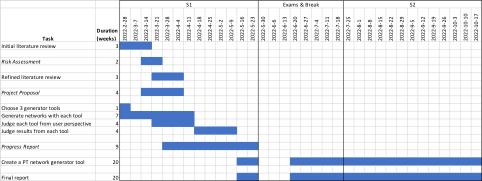
\includegraphics[width=.9\linewidth]{./img/timeline.png}
\captionof{figure}{\label{fig:timeline}Project timeline}
\end{center}
\subsection{Risk management}
\label{sec:org02e56c3}
\label{app:B}

\begin{center}
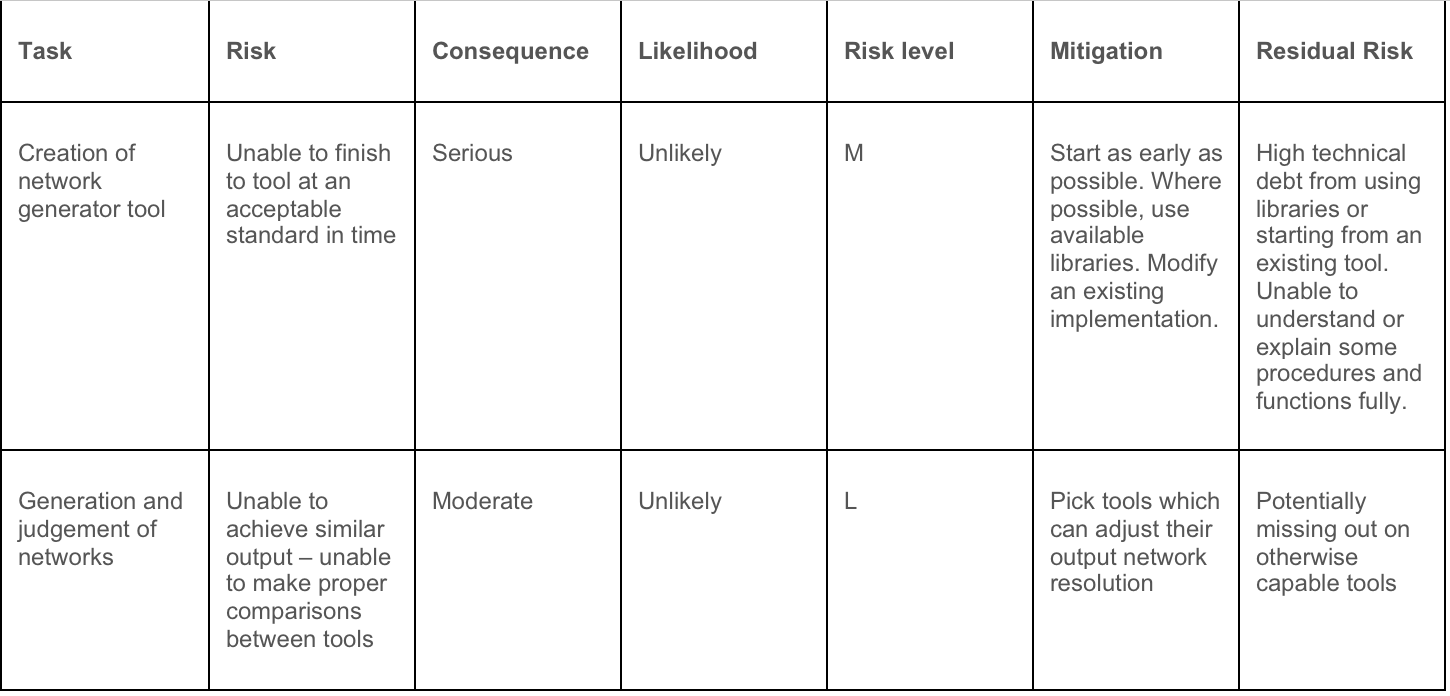
\includegraphics[width=.9\linewidth]{./img/risk.png}
\captionof{figure}{\label{fig:risk}Risk management plan}
\end{center}
\end{document}
